\documentclass{article}

\usepackage{siunitx} % Provides the \SI{}{} and \si{} command for typesetting SI units

\usepackage{graphicx} % Required for the inclusion of images

\usepackage{tabularx} % Tables

\usepackage{natbib} % Required to change bibliography style to APA

\usepackage{amsmath} % Required for some math elements

\usepackage{hyperref} % To include links

% Many options for pseudocode
\usepackage{algorithm2e}
\usepackage{algorithmic}

\usepackage{listings} % Python code blocks

\setlength\parindent{0pt} % Removes all indentation from paragraphs

\title{Lab \#3 Report: Wall-Following on the Robot} % Title

\author{Team \# 6\\\\ Sera Hamilton \\ Carlos Sanchez \\ Yuewei Liu \\ Miguel Padilla \\ \\ RSS} % Team # + Names, Class (RSS)

\date{\today} % Date for the report

\begin{document}

\maketitle

\section{Introduction}

This lab required the design and implementation of an autonomous wall-following robot with two high level goals in mind:
\begin{itemize}
    \item Designing a safety controller to prevent the robot from crashing if it's predicted trajectory is deemed dangerous
    \item Design a controller that keeps robot a desired distance away from the wall
\end{itemize}

Before approaching these tasks, we used our simulated wall-follower as a launch pad for getting real-time data from the LIDAR sensor. This data serves as the primary input to our controllers and needed to be extracted and interpreted very carefully. Developing the safety and wall-follower controllers followed naturally.\\

For the safety controller, we designed a system that stopped the drive signal of the robot when the estimated position of the wall was expected to intersect with robot's path. More precisely, the safety controller design depends on the distance of the robot from the wall and it's velocity.\\

Our team implemented a Proportional-Derivative (PD) Controller that tracks the error between the robot’s desired distance from the wall and the measured distance. We experimentally determined our control values, $K_P$ and $K_D$, which contributed to the proportional and derivative components, respectively.\\

   

% \end{list}


\section{Technical Approach}
Our technical approach can be broken down into two different goals, the first being the design of the safety controller, and the second the wall follower, both implemented using ROS2. Our pipeline is shown in figure 1 below.

\begin{figure}[!h]
    \centering
    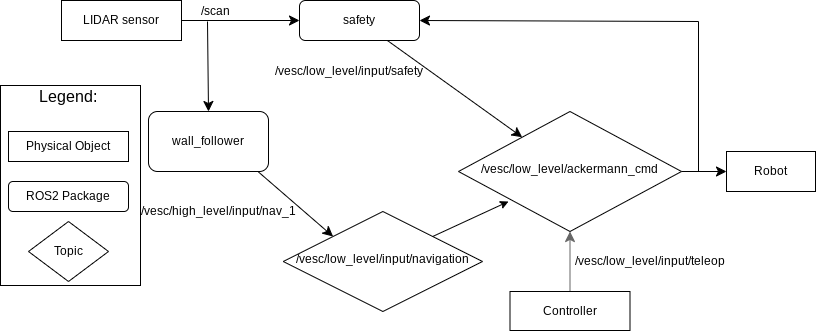
\includegraphics[width=\linewidth]{lab3diagram.drawio.png}
    \caption{Diagram of the ROS2 controllers and relevant topics. The higher precedence of safety goal than that of the wall-following goal is reflected in the fact that the \textit{safety} topic has higher precedence than the \textit{navigation} topic, just as the \textit{teleop} topic has higher precedence than the \textit{safety}.}
    \label{fig:enter-label}
\end{figure}


\subsection{Safety Controller}
To maintain safety of the car, we needed to design a controller that prevents the car from collision. This warranted a general approach of processing the LIDAR scans in front of the robot and using their ranges to determine when to stop. Further, we wanted to make the controller robust to velocity changes, thus we decided to make the stopping distance linearly depend on the velocity.\\

In a simple initial approach, we fit a line to all points within a 40° range in front of the robot and used the closest point on that line as the reference distance, as shown in Figure 2. If this was less than the threshold (equal to half the velocity), the safety controller would stop the car. \\
\begin{figure}[!h]
\begin{center}
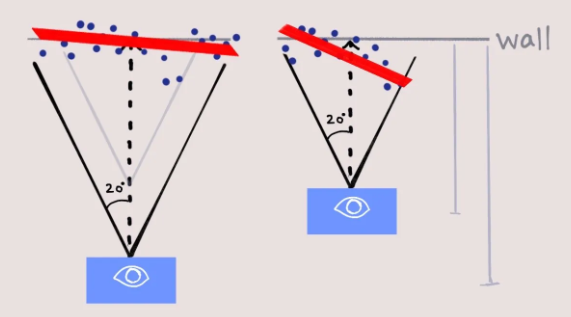
\includegraphics[width=0.7\textwidth]{safety_all.png}
\caption{On the left, we have the expected behavior of least-squares regression on all of the points within the field of view (fov). On the right is a common problem we encountered in complex situations that would cause unpredictable behavior from the safety controller: sometimes behaving too strong and at other times too weak.}
\end{center}
\end{figure}

However, while this worked well for smooth walls, because we were fitting a line to all of the points in front of the car we ran into issues when there was greater variance in the distance of the obstacles picked up by the car.\\

We also noticed issues when operating in more complex environments (like in a classroom, where the most common thing at the robot's eye-level are the legs of the tables and chairs), so we understood that the safety controller needs to be activated on a smaller number of points. Using the least-squares estimate on all the scans was over-generalizing the possibility of more complex environments down to an assumption of the existence of a flat wall. After speaking as a team, we decided that we needed to try a simpler metric. \\

The safety controller needed to operate only on the closest obstacles. Taking this idea into account, we update the controller to use the 10th percentile distance as the closest obstacle distance, which was then compared to the threshold, as demonstrated in Figure 3.
\begin{figure}[!h]
\begin{center}
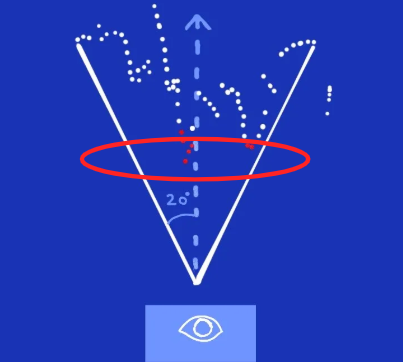
\includegraphics[width=0.3\textwidth]{safety_10th.png}
\caption{The 10th percentile distance of the 40$^\circ$ fov in front of the robot minimized the amount of LIDAR points that needed to be ``too close" for the safety controller to command the robot to stop.}
\end{center}
\end{figure}

More formally, let the 10th percentile distance be $d_{10th}$ and the threshold distance be $d_{thresh} = 0.5 * v$ where $v$ is the car's velocity. If $d_{10th} < d_{thresh}$, we command a velocity of 0 to the car, telling it to stop.

\subsection{Wall Follower}
The main objective was to develop a robust algorithm to cause the car to follow a wall. In considering this, we wanted to create a wall follower that was able to operate in many scenarios with different obstacle geometries, velocities, and distances from the wall.\\

To accomplish a robot that follows at a reference distance $r$, we set up a Proportional Derivative (PD) controller. We decided that the system was simple enough to use PD instead of more complicated methods. Additionally, we decided to leave out the integral term in our approach after observing how the system behaved without it, concluding that it was not necessary as the steady state error was quite low.\\ 

\subsubsection{Controller Design}
As shown in the block diagram below, we calculate an error $e(t) = r - y(t)$, where the measured output $y(t)$ is the robot's current wall distance, whose calculation is elaborated upon under section 2.2.2 Wall Estimation. We estimate the derivative of the error $\dot{e}(t) = \frac{e(t) - e(t-1)}{\Delta t}$ based on the previous error, the current error, and the change in time. From this, we can calculate our steering input $u(t) = K_pe(t) + K_D\dot{e}(t)$ to feedback into the controller.\\\\
\begin{figure}[!h]
\begin{center}
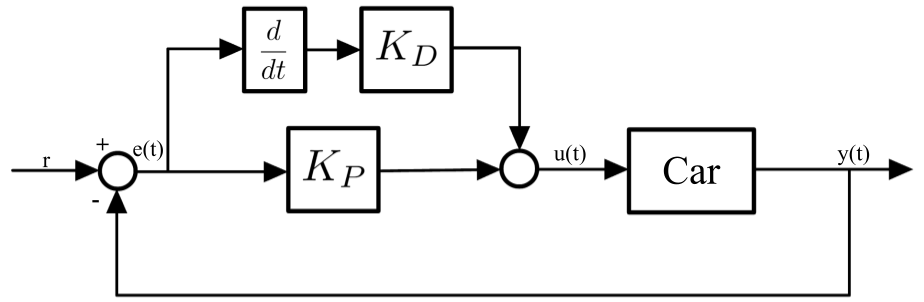
\includegraphics[width=0.9\textwidth]{block_diagram.png}
\caption{A block diagram of the PD controller we implemented for our wall follower representing the equation $u(t)=K_Pe(t)+K_D\dot{e}(t)$.}
\end{center}
\end{figure}

To determine the gains we initially increased $K_P$ until a reasonable rise time was observed with some oscillation. To lessen the oscillations and overshoot, we then increased $K_D$ until we had a desired damping that allowed the system to converge to a steady state with a low settling time and overshoot. Our final gains were $K_P = 2.0$ and $K_D = 1.5$, which allowed us to reliably follow the wall at a set distance along with handling uneven geometry or corners. \\ 

\subsubsection{Wall Estimation}
Our approach to wall estimation can be broken down into three parts. First, we slice the full list of ranges into the relevant angles to consider depending on the side the car is following. Testing the car, we determined that the range of angles to pull for the left was $[-\frac{\pi}{20}, \frac{\pi}{2}]$ and similarly for the right  $[\frac{\pi}{20}, -\frac{\pi}{2}]$, as shown in the below image.\\

\begin{figure}[!h]
\begin{center}
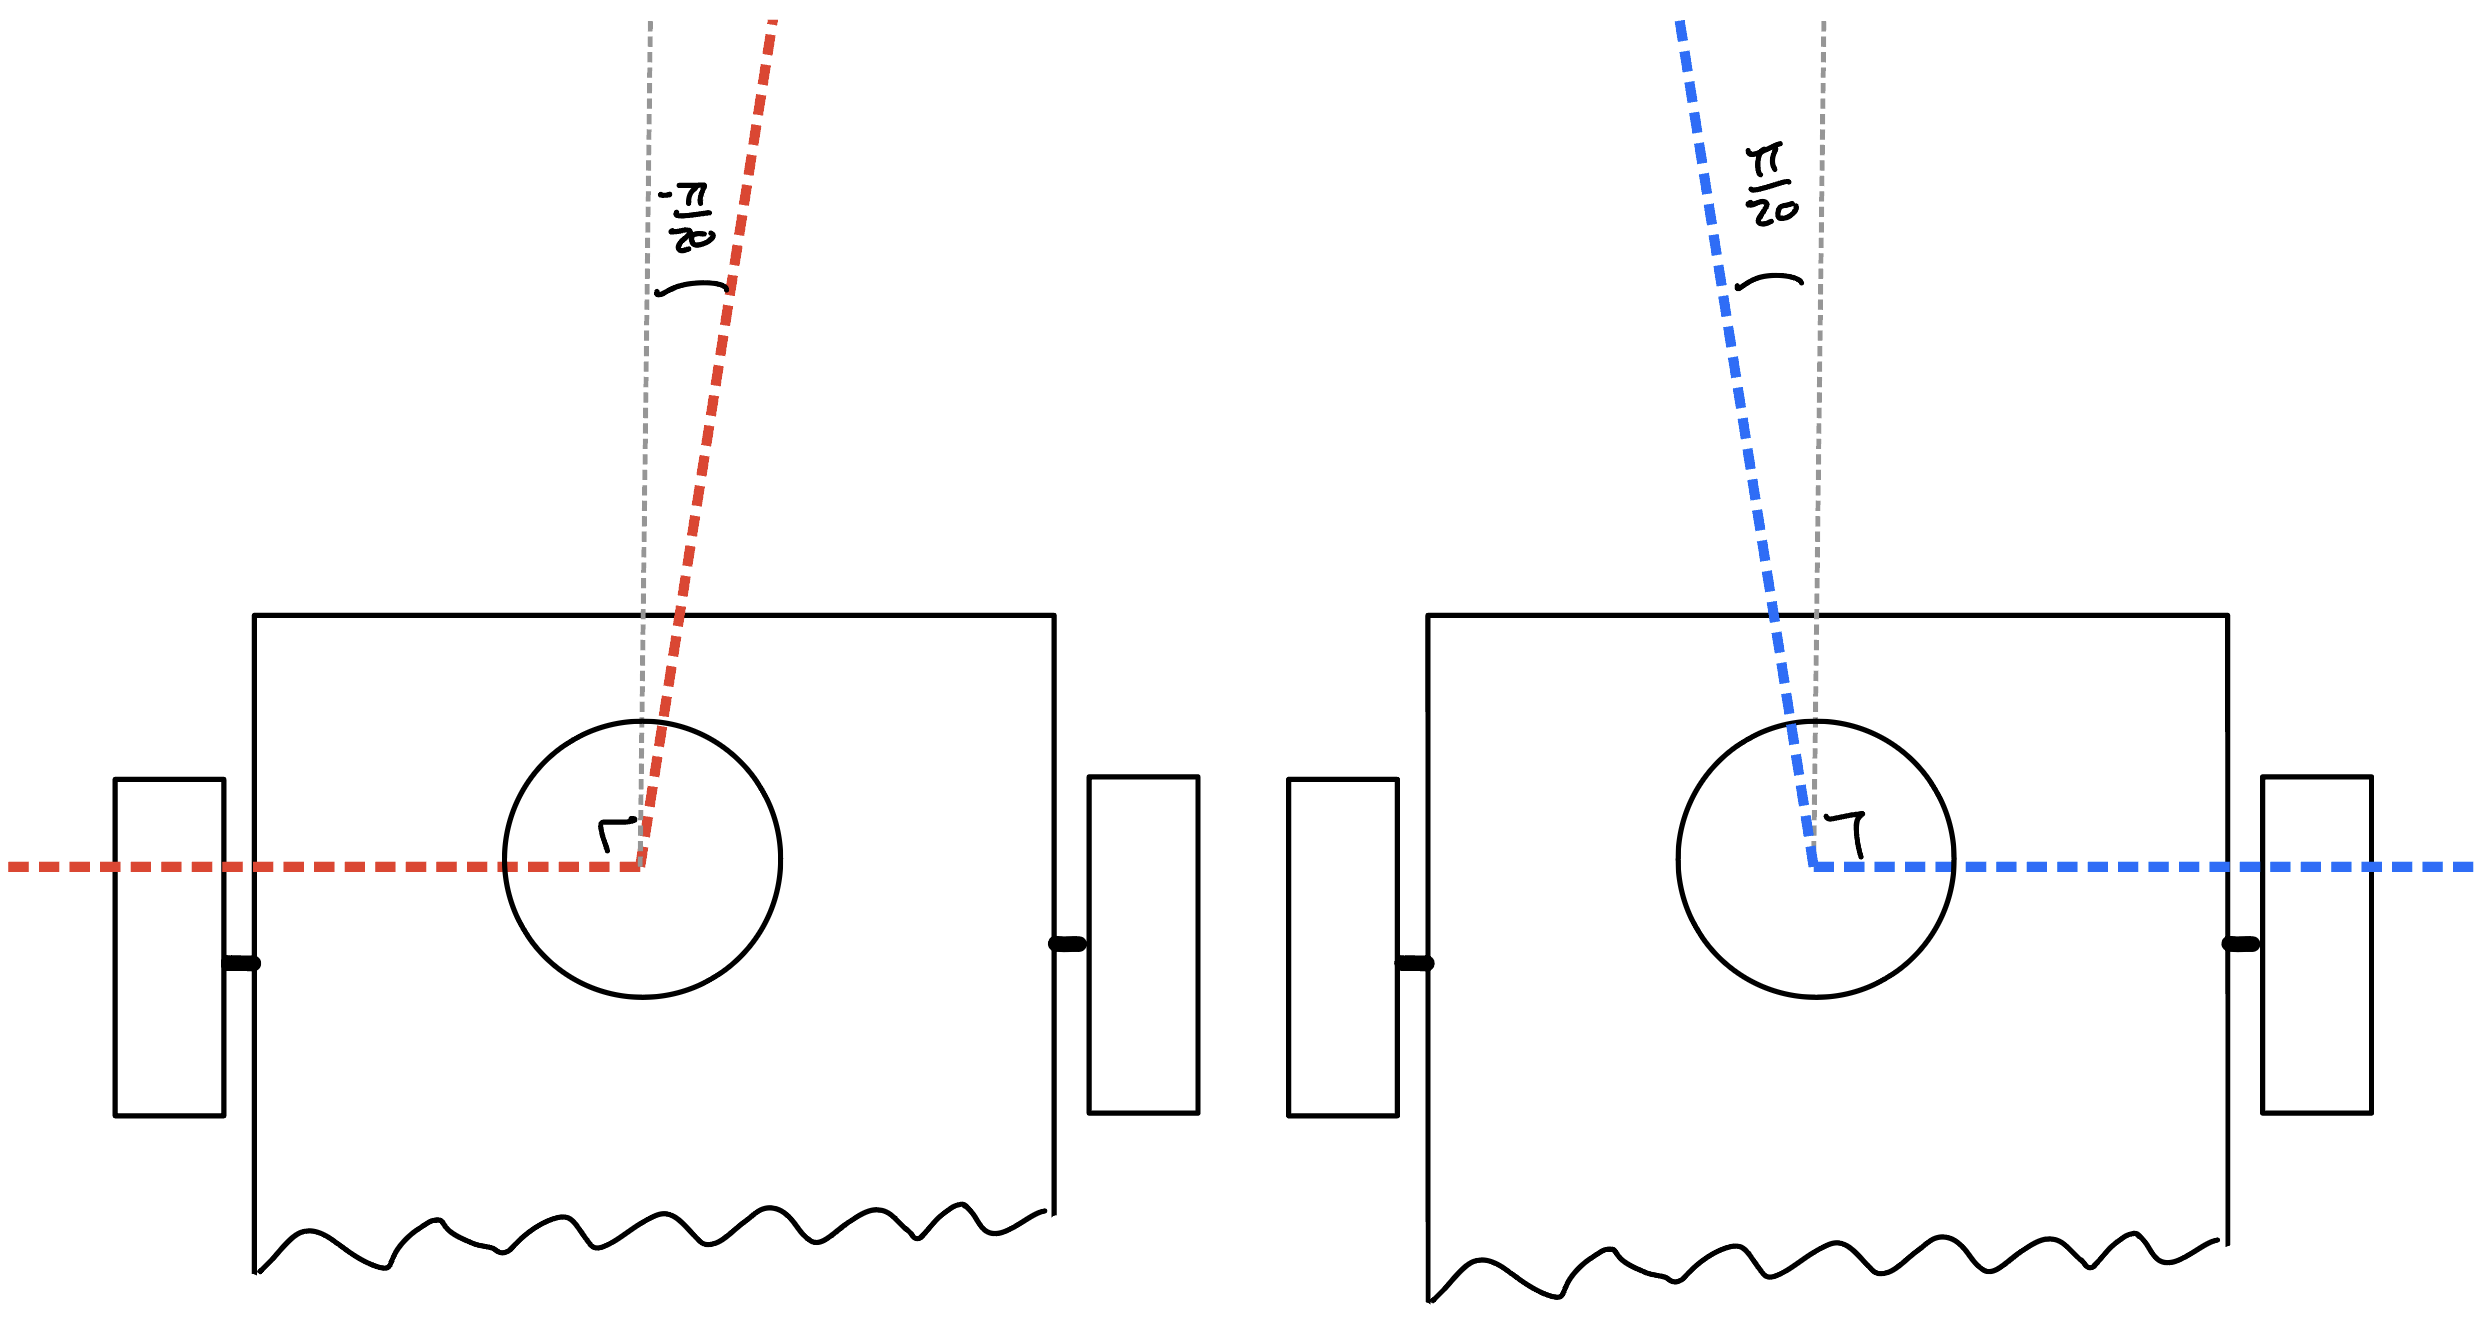
\includegraphics[width=1.0\textwidth]{car_wall_ranges.png}
\caption{Demonstration of the left fov angles $[-\frac{\pi}{20},\frac{\pi}{2}]$ and right fov angles $[-\frac{\pi}{2},\frac{\pi}{20}]$ on their respective sides of the image.}
\end{center}
\end{figure}

Second, similar to the safety controller, we further constrain the data to only include points within a distance threshold, equal to the 50th percentile range. This was done to solve the issue of incorrect wall fitting in wide open spaces, demonstrated in Figure 6 below. \\

\begin{figure}[!h]
\begin{center}
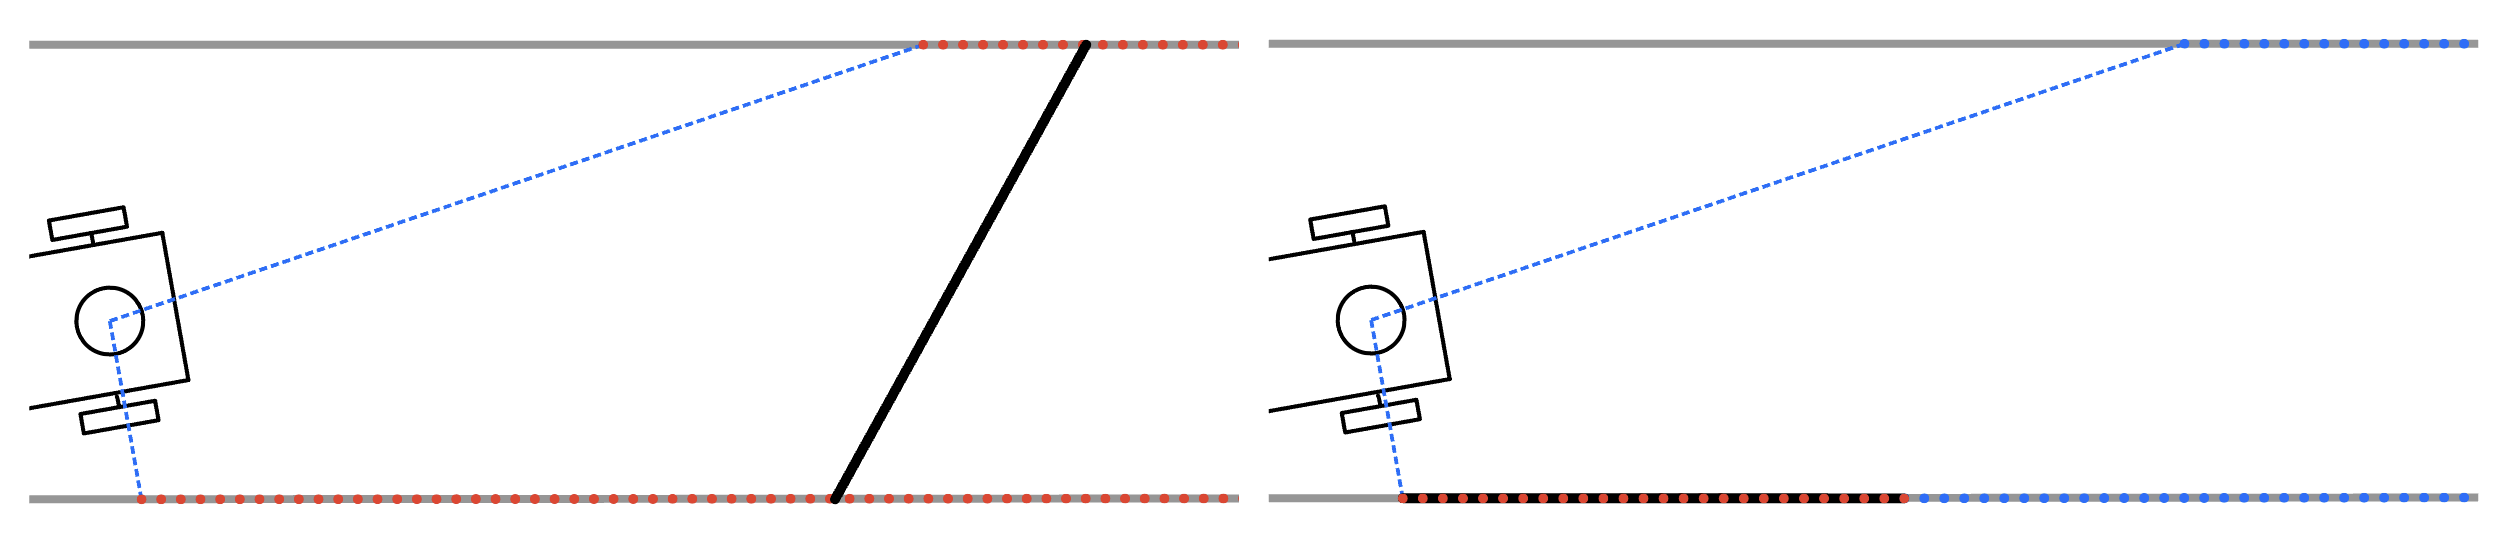
\includegraphics[width=\textwidth]{wall_percentile.png}
\caption{Similar to our safety controller in 2.1, we have a percentile metric to limit far-field outliers from contaminating the LIDAR data. The left image demonstrates the line (in black) that would be fit when considering all the visible points (in red) without the threshold. On the right we have the line that is fit when considering only those points within the threshold.}
\end{center}
\end{figure}

Finally, we use least squares to fit a line to these points, also demonstrated in Figure 6. With this, we have a wall estimate, and can calculate our current distance $r$ using the orthogonal projection of the least squares fit line on the origin (i.e. the center-point of our robot).\\

Bringing this all together, we end up with the following display in RVIZ when we are following the wall straight on.\\

\begin{figure}[!h]
   \begin{minipage}{0.55\textwidth}
     \centering
     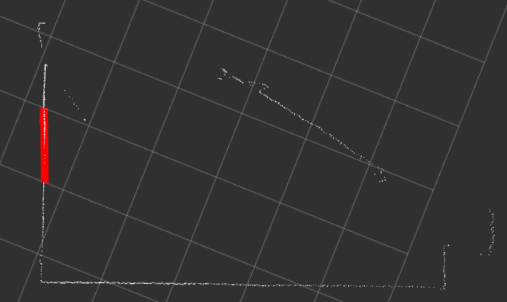
\includegraphics[width=1.0\linewidth]{scan_straight_rviz.png}
   \end{minipage}
   \begin{minipage}{0.45\textwidth}
     \centering
     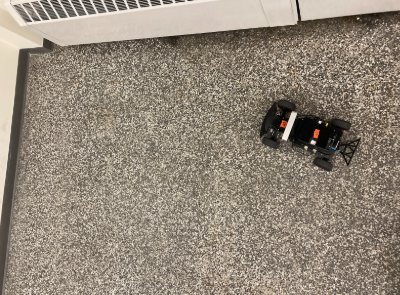
\includegraphics[width=1.0\linewidth]{scan_straight_car.png}
   \end{minipage}
   \caption{The red line in RVIZ is a drawing of the least-squares lines projected on top of the LIDAR points that are being read by the sensor. NOTE: the size of the line is limited to that of the fov of the wall following side (in this case, on the right side).}
\end{figure}

Later, while turning to avoid the corner, we get the following.

\begin{figure}[!h]
   \begin{minipage}{0.53\textwidth}
     \centering
     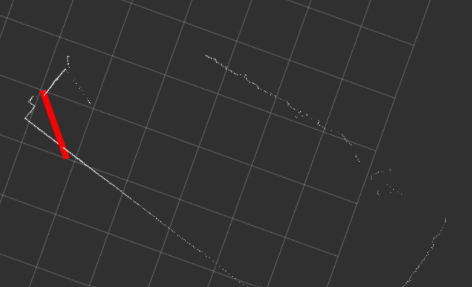
\includegraphics[width=1.0\linewidth]{scan_turn_rviz.png}
   \end{minipage}
   \begin{minipage}{0.47\textwidth}
     \centering
     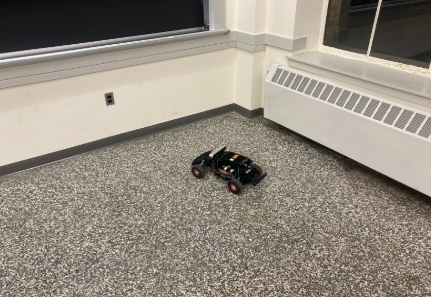
\includegraphics[width=1.0\linewidth]{scan_turn_car.png}
   \end{minipage}
   \caption{As the robot drives up to a corner, the angle of the least-squares approximation increases. This increases the calculated error of the robot to then correct course by changing the steering angle.}
\end{figure}

To get a better look at the behavior of the car with our controller from 2.2.1, visit \href{https://drive.google.com/file/d/1FpQVgkOg14kKm138I-bZFko9YBxphWZr/view?usp=drive_link}{this link}.

\pagebreak
\section{Experimental Evaluation}


Our experimentation and evaluation process consisted of 3 primary components including small-scale baseline tests for debugging, qualitative metrics such as performance on common obstacles, and finally a quantitative analysis of error based on LiDAR data.\\


One baseline test we utilized was presenting a “wall” at varying distances to test the safety controller by observing if the car reacted correctly to the presented obstacle, and if the distances read back reflected the reality. We verified the distance measurements estimated by the LiDAR and wall estimation algorithm by checking against the known distance of the obstacles presented. These obstacles were presented stationary, as well as dynamically, to test the car’s ability to react safely to obstacles moving relative to it. We concluded our mini tests only when our car was able to reflect distances accurately and consistently to within a centimeter of actual distance, and was robust against sudden movements.
Our quantitative analysis process is detailed below:\\

We tested the wall-following PD controller by tracking the robot's error as a function of time. We define error as the difference between the robot’s actual distance from the wall vs its desired distance from the wall. When the robot has to turn to adjust, we can visualize how long it takes for the robot to return to the desired distance. \\

We experimented with a variety of desired distances and speeds for the robot as detailed below. \\

\subsection{Desired Distance = 1 m, Speed = 1 m/s}
For this test we started the robot at a distance greater than the desired distance and we followed the right wall.
When the desired distance was 1m and the speed of the robot was 1 m/s, the robot drove aggressively towards the right wall to correct the initial error. We can see this reflected in the large dip at the beginning of the plot. The robot then corrects itself causing the subsequent spike in the error plot, which demonstrates the overshoot of the controller. From there, the robot oscillates slightly around the 0 error mark, which indicates it is very close to 1m from the right wall. This behavior repeats a second time in this plot due to a protrusion in the wall on which we tested. However, after this second spike at around the 380 timestamp, the robot is again able to correct and oscillate slightly around 0 error.
\begin{figure}[!h]
\begin{center}
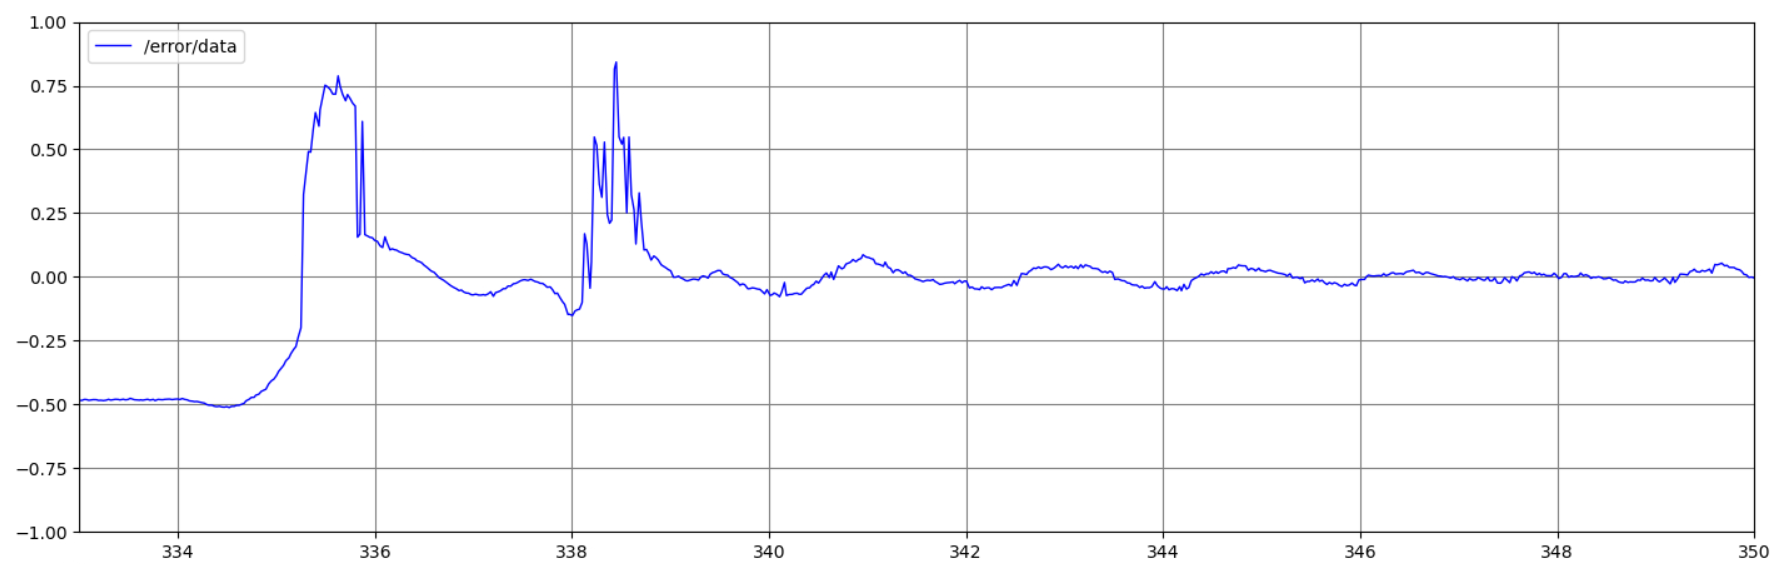
\includegraphics[width=\textwidth]{error_speed_1_dist_1.png}
\caption{Error vs time for a distance of 1 meter and speed of 1 m/s.}
\end{center}
\end{figure}

\subsection{Desired Distance = 1 m, Speed = 1.25 m/s}
For this test, we set the desired distance to 1m and the speed to 1.25 m/s. We found a flatter section of wall to work with and started the robot at around the desired distance. We then tracked the robot's error as we did before. Since the robot had very little correction to perform, the error can be seen hovering around 0. As mentioned, this wall was flatter than the previous and exhibited the expected behavior of little to no overshoot.
\\\\
\begin{figure}[!h]
\begin{center}
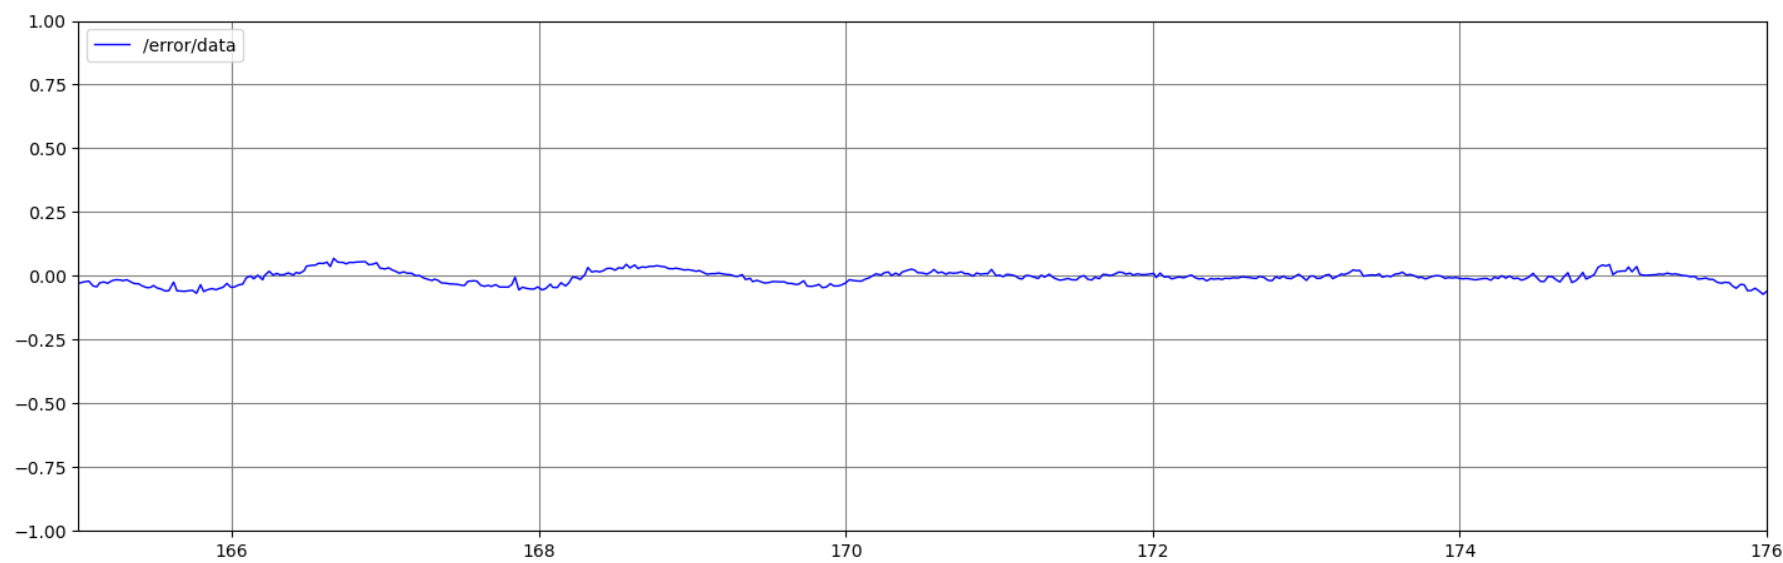
\includegraphics[width=\textwidth]{error_speed_1_dist_125.png}
\caption{Error vs time for a distance of 1.25 meters and speed of 1 m/s along a smooth wall.}
\end{center}
\end{figure}

\subsection{Desired Distance = 1.5 m, Speed = 1.25 m/s}
For this test, we set the desired distance to 1.5m and the speed to 1.25 m/s. We tested on a bumpier wall and observed the error over time. The expected behavior holds for this test as it did for the previous two, only now there are more point of correction that the robot needs to make. This is reflected in the spikes of this error plot.
\begin{figure}[!h]
\begin{center}
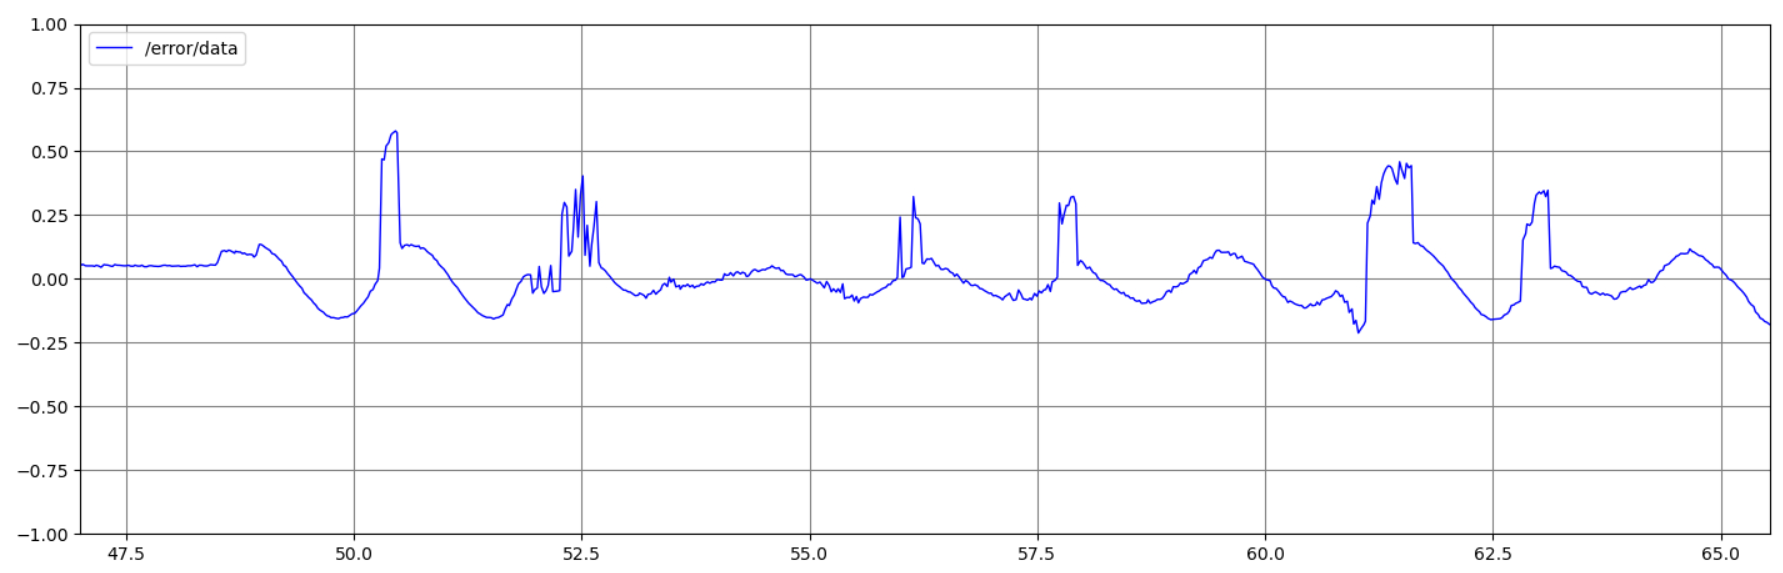
\includegraphics[width=\textwidth]{error_speed_15_dist_125.png}
\caption{Error vs time for a distance of 1.5 meters and speed of 1.25 m/s along a bumpier wall.}
\end{center}
\end{figure}

Our qualitative testing was less rigorous. We observed visually how the robot reacted to imperfections in the wall, and how it was able to handle turns (which are nothing more than changes in the wall geometry). From our recorded videos, we are able to see a representation of our error plot’s in physical form. When the robot corrects, there is some overshoot and subsequent oscillations. We have provided a \href{https://drive.google.com/file/d/1AO_3WzXyMMgyawGHh4i-X2u07TG5eoCh/view?usp=sharing}{link} our video test.

% One baseline test we utilized was presenting a “wall” at varying distances to test the safety controller by observing if the car reacted correctly to the presented obstacle, and if the distances read back reflected the reality. We verified the distance measurements estimated by the LiDAR and wall estimation algorithm by checking against the known distance of the obstacles presented. These obstacles were presented stationary, as well as dynamically, to test the car’s ability to react safely to obstacles moving relative to it. We concluded our mini tests only when our car was able to reflect distances accurately and consistently to within a centimeter of actual distance, and was robust against sudden movements.

% One challenge we encountered in real life testing of the safety controller in basement tunnels was the inconsistent performance on irregular geometry, especially with differently angled walls and  thin chair or table legs. Furthermore, the car sometimes struggled with incorrect LiDAR data which often detected points tens of meters away, even while the car directly faced a wall. We adjusted parameters such as target stopping distance and field of view angle. We also introduced absolute and percentile based thresholding to eliminate outlier values. To determine optimal values for these parameters and determine the superior method of thresholding, we qualitatively compared performance of the car on common obstacles like angled walls, concave and convex corners, and various irregular geometry. 

% In particular, we found that percentile based thresholding (10th percentile, keeping only the closest points) was ideal for identifying obstacles relevant to safety control. Furthermore, through trial and error, we determined that the minimum safe stopping distance was 25 centimeters. Greater distances resulted in severe jittering of the curve fit due to the noisy LiDAR data and limited points included in the set 20 degree field of view, resulting in inconsistent controls and shaky car movement. 

% Introducing point thresholding for the safety controller also was found experimentally to make the car robust against thin obstacles like microphone stands, chair legs, and table legs. Rather than being distracted by walls or objects in the background, our wall follower generates trajectories from the 50th percentile of LiDAR scan points and operates its safety controller using the 10th percentile of scanned points (thus eliminating outliers along the way.)



\section{Conclusion}

In this design phase, we successfully developed and implemented a wall-following robot. We focused on two key components: the safety controller and the wall-following controller. The safety controller, which prevents the robot from colliding with obstacles, was designed using LIDAR data and velocity-dependent stopping thresholds. We refined the safety controller by applying percentile-based distance thresholds, which enhanced its robustness in a variety of scenarios.
\\\\
For the wall-following controller, we implemented a Proportional-Derivative (PD) controller, which ensured the robot maintained a consistent distance from the wall. We tuned the PD controller's gains based on experimental results, allowing the robot to reliably follow the wall. The system was tested using both simulated and real-world data, demonstrating its ability to perform in various scenarios.
Moving forward we could further optimize the efficacy of both controllers. 
\\\\
Specifically, the safety controller can be improved to handle more complex environments and the wall-following controller could be improved to adjust quickly to diverse wall shapes. Additionally, we can perform further testing in more challenging scenarios such as highly cluttered environments and at varying speeds and desired distances. In the next lab, we plan to abstract some of our wall-following to a new design challenge: detecting objects and driving towards them.


\section{Lessons Learned}
\subsection*{Sera Hamilton}
When we were first introduced to the lab I felt like there were so many different tasks to complete and was wondering how to best manage the work, especially when working with a team of people who I didn't know so well. Through this lab I learned how to first break a problem down into multiple steps. I think the CI lectures on consensus decision making and working in teams really helped us first define the problem, come up with ideas on how to tackle it, and then implement it. I learned how to break things down into steps, to focus first on one task, such as the safety controller, then the wall follower, then the briefing and finally the report. And similarly, when problems arose (such as incorrect wall following behavior), to take a step back as a team to first break down possible issues, come up with a few possible solutions, and then finally deciding on one we all agree on to initially test out. Through this process of learning how to tackle a larger project I also learned how to work with a new team and put trust into my team members so that even if I or the group didn't have an immediate solution to a problem, I could trust us to work together to figure out an answer.

\subsection*{Carlos Sanchez}
This lab required our team to work with an iterative process, both in the testing/experimental phase and in the design decision phases. When working on the technical components we reached points of contention about the best possible choice to implement and there were often a number of ideas. We were able to test them and reach an agreement about which one we felt was most viable. This goes to show how valuable it is to work with a group of minds (rather than just my own) and how important it is to consider multiple potential directions. In addition, presenting technical work in a visual manner is somewhat new to me. It was a bit challenging to figure out where to start and what to include in the presentation/paper. However, the CI lectures were helpful in providing guidance on this process. I learned that it is important to first zoom out and demonstrate a high-level overview of the work we did. Then, step by step, we can show the more precise aspects of the process, detailing the technical side. Overall, this was a challenging but valuable learning process, and I feel better prepared to create new projects.

\subsection*{Yuewei Liu}
In this lab, I learned a lot about both the technical aspects and teamwork necessary for this project. On the technical side, my biggest lesson was how making the transition from a simulated environment to real hardware can be surprisingly challenging. We ran into a lot of unexpected issues at first, but thanks to our ability to work together at a team, I don’t think it ended up affecting too much about our actual wall follower. I was also reminded just how important communication is to a functioning team. I felt that my team was able to work together very effectively because we were very diligent about documenting progress, communicating changes in plans, and scheduling times to meet. Additionally, I learned a lot about how to debug and analyze problems with a system based on feedback in the form of reading back sensor values and in particular on this lab, checking what the car was seeing on RViz. This form of debugging integrating both hardware and software was new to me.

\subsection*{Miguel Padilla}
Throughout this lab, I found myself wondering what the ratio of work is between solving the technical aspects of the lab to the communication aspects. I expected to spend much more time with the technical aspects of the lab (probably, more like hoping to) because wall-following felt like a more complex goal than its proven to be (before starting on the labs), but I've found myself spending more time on the communication aspects: the briefing and the report. The time it takes to process the ideas and data that result from a lab can feel never-ending, something can always be displayed or conveyed better. In that way, technical communication feels much more like an art than a science. Sometimes it just takes multiple design iterations of a diagram to get a sense of what is not yet being communicated by a visual, that may be critical for the audience's understanding.

\end{document}